% !TeX TS-program = xelatex
% !TeX encoding = UTF-8

\documentclass[11pt, a4paper]{article}
\usepackage[utf8]{inputenc}
\usepackage{graphicx}
% 字体设置
\usepackage{xeCJK}
\setCJKmainfont[BoldFont=SimHei,ItalicFont=KaiTi]{SimSun}
\setCJKmonofont{SimSun}
\setCJKsansfont{SimSun}
% 页面设置
\usepackage{indentfirst}



% 数学记号
\usepackage{amsmath,amssymb,amsthm,amsfonts}
\usepackage{bm}
\DeclareSymbolFont{cmsymbols}{OMS}{cmsy}{m}{n}
%\SetSymbolFont{cmsymbols}{bold}{OMS}{cmsy}{b}{n}
\DeclareSymbolFontAlphabet{\mathcal}{cmsymbols}
% 自定义数学记号在这里
\newcommand{\mat}[1]{\bm{#1}}
\newcommand{\argmax}[1]{\underset{#1}{\operatorname{argmax}}}
\newcommand{\argmin}[1]{\underset{#1}{\operatorname{argmin}}}
\newcommand{\inR}[1]{\in\mathbb{R}^{#1}}
\DeclareMathOperator{\svd}{SVD}


% 算法环境
\usepackage{algorithm}
\usepackage{algorithmic}
\usepackage{eqparbox}
\renewcommand\algorithmiccomment[1]{%
	\hfill\#\ \eqparbox{COMMENT}{#1}%
}
\usepackage{etoolbox}  % patch def of algorithmic environment
\makeatletter
\patchcmd{\algorithmic}{\addtolength{\ALC@tlm}{\leftmargin} }{\addtolength{\ALC@tlm}{\leftmargin}}{}{}
\makeatother
\renewcommand{\algorithmicrequire}{\textbf{输入:}}
\renewcommand{\algorithmicensure}{\textbf{输出:}}


% 杂七杂八
\usepackage{lmodern}
\usepackage[T1]{fontenc}
\usepackage{titlesec}
\usepackage{titling}
\usepackage{verbatim}
\usepackage{float}
\usepackage{enumerate}
\usepackage{enumitem}
\usepackage{amsthm}
\usepackage{graphicx,wrapfig,lipsum}
\usepackage[usenames,dvipsnames]{color}
\usepackage{xcolor}
\usepackage{tikz}
\usepackage{hyperref}
\usepackage{caption}
\usepackage{subfig}
\usepackage{microtype}
\usepackage{cleveref}
\usepackage{textcomp}

\colorlet{inlinkcolor}{green!50!black}
\colorlet{exlinkcolor}{red!50!black}
\hypersetup{
	colorlinks=false,
	frenchlinks=false,
	pdfborder={0 0 0},
	naturalnames=false,
	hypertexnames=false,
	breaklinks,
	colorlinks = true,
	allcolors = inlinkcolor,
	urlcolor = exlinkcolor,
}


% 代码
\usepackage{listings}


%\lstloadlanguages{Matlab}
\lstset{language=Matlab,
	frame=single,                           % single framed
	basicstyle=\small\ttfamily,
	keywordstyle=[1]\color{Blue}\bfseries,  % primitive funs in bold blue
	keywordstyle=[2]\color{Purple},         % args of funs in purple
	keywordstyle=[3]\color{Blue}\underbar,  % user funs in blue with underbar
	stringstyle=\color{Purple},             % strings in purple
	showstringspaces=false,
	identifierstyle=,
	commentstyle=\usefont{T1}{pcr}{m}{sl}\color{DarkGreen}\small,
	tabsize=4,
	% more standard MATLAB funcs
	morekeywords={sawtooth, square},
	% args of funcs
	morekeywords=[2]{on, off, interp},
	% user funcs
	morekeywords=[3]{FindESS, homework_example},
	morecomment=[l][\color{Blue}]{...},     % line continuation (...) like blue comment
	numbers=left,
	numberstyle=\tiny\color{Blue},
	firstnumber=1,
	stepnumber=1
}


% 环境中文化
\floatname{figure}{\texttt{图}}
\floatname{table}{\texttt{表}}
\floatname{algorithm}{\texttt{算法}}

\theoremstyle{plain}
\newtheorem{theorem}{\texttt{定理}}
\crefname{theorem}{定理}{定理}
\Crefname{theorem}{定理}{定理}

\theoremstyle{plain}
\newtheorem{lemma}{\texttt{引理}}
\crefname{lemma}{引理}{引理}
\Crefname{lemma}{引理}{引理}

\theoremstyle{plain}
\newtheorem{corollary}{\texttt{推论}}
\crefname{corollary}{推论}{推论}
\Crefname{corollary}{推论}{推论}

\theoremstyle{definition}
\newtheorem{definition}{\texttt{定义}}
\crefname{definition}{定义}{定义}
\Crefname{definition}{定义}{定义}

\theoremstyle{remark}
\newtheorem*{remark}{\texttt{备注}}
\crefname{remark}{备注}{备注}
\Crefname{remark}{备注}{备注}

\theoremstyle{definition}
\newtheorem{example}{\texttt{例}}
\crefname{example}{例}{例}
\Crefname{example}{例}{例}

\crefname{equation}{\textsf{公式}}{\textsf{公式}}
\Crefname{equation}{\textsf{公式}}{\textsf{公式}}

\crefname{algorithm}{\texttt{算法}}{\texttt{算法}}
%\Crefname{algorithm}{alg}{alg}

\renewcommand\qedsymbol{$\blacksquare$}	
\renewcommand*{\proofname}{\texttt{证明:}\nopunct}
\usepackage{xcolor}

\newcommand{\T}[1]{\texttt{#1}}
\newcommand{\nl}{\newline}
\newcommand{\red}[1]{\textcolor{red}{#1}}
\newcommand{\blue}[1]{\textcolor{blue}{#1}}
\newcommand{\s}{\footnotesize}

\usepackage{fancyhdr}
\renewcommand{\abstractname}{\large \T{摘  要}}
\usepackage[nottoc,notlof,notlot]{tocbibind} 
\newcommand{\Page}{
	\thispagestyle{fancy}
	\rhead{}
	\chead{\T{“高等数值算法与应用”期末Project报告(2020年秋季学期)}}
}

\pagestyle{fancy}
\fancyhf{}
\chead{\T{“高等数值算法与应用”期末Project报告(2020年秋季学期)}}
\rfoot{\T{第}\thepage\T{页}}
\usepackage{multirow}



\begin{document}
	
\title{大规模稀疏矩阵迭代解法研究报告}
\author{\T{郭文韬, 刘志强}}
\date{\T{2021年1月13号}}
\maketitle
\Page

\begin{abstract}
	
\end{abstract}

{\bf \textbf{\T{关键词:}} \T{预条件子}, \T{多级}, \T{低秩修正}, \T{舒尔补}, \T{矩阵稀疏化}, \T{图分割}


\section*{\T{引言}}
% 1
\T{
	矩阵的求解($A x = b$)一般分为直接解法和迭代解法。 对于小规模的矩阵,人们一般采用LU分解(对于一般稠密矩阵,当然也有选主元等增加算法稳定性的方法),Choleskey分解(对于对称正定矩阵)等方法, 迭代解法更适用于大规模的稀疏矩阵。 常用的迭代解法有Jacobi迭代,高斯-赛德尔迭代,逐次超松弛法(SOR方法,以及用于对称矩阵的SSOR),预处理共轭梯度(PCG)等方法。
}\cite{Iter}
\\
\T{
	迭代解法的收敛速度一般难以确保,经常需要人为添加“预条件子”来加快收敛速度。常见的预条件技术可以被分为三大类: 
}

\T{
	$M^{-1} A x = M^{-1} b$,
	$A M^{-1} u = b, x = M^{-1} u$,
	$M_L^{-1} A M_R^{-1} u = M_L^{-1} b, x = M_R^{-1} u$。使用预条件子可以降低迭代矩阵的2-条件数来提高迭代的收敛速度和解的准确性,在实际运用中经常可以和PCG,GMRES等方法有效结合。
}

\T{	
	传统的预条件子有(块)Jacobi预条件子, 高斯-赛德尔预条件子,SOR(SSOR)预条件子,也有给不完全Choleskey分解/不完全LU分解的预条件子。在迭代算法中,例如块Jacobi迭代适合于并行的实现,但其他的迭代算法未必适合。类似地,我们也希望预条件子的计算也尽可能支持并行。
}

\T{Y. Saad提到}\cite{Course}\T{一些工业界支持并行的预条件子有Schwarz,基于舒尔补的,以及多级ILU类的预条件子。 在本论文,我们主要探讨了基于舒尔补的预条件子和多级低秩修正的ILU/IC预条件子。}\T{我们也采用了domain-decomposition技术}\cite{MLR}\T{对矩阵进行划分边界/内部节点然后使用metis包做图切割}

\section{\T{多级低秩修正预条件子方法 (MLR)}}
\subsection{\T{图分割}}
\T{我们知道块Jacobi预条件子M = $\text{diag}(A_{11}, \ldots, A_{nn})$ 易于并行,但假如对对角块做完全分解则消耗内存大,假如做不完全分解迭代步数还是会很高, 但对于$A = \begin{bmatrix} A_{11} & A_{12} \\ A_{21} & A_{22} \end{bmatrix}$, 我们可以选$B = \begin{bmatrix} A_{11} & \\ & A_{22} \end{bmatrix}$, 然后做一个低秩近似使得 $M^{-1}=B^{−1}+LRC$
}


\begin{figure}[H]
	\label{domain}
	\caption{\T{图分割-对边切割}\cite{MLR}}
	\centering
	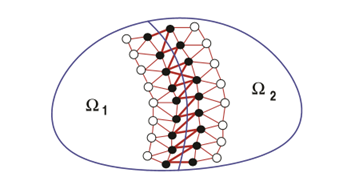
\includegraphics[width=200pt,height=100pt]{graph.png}
\end{figure}

\T{我们先对稀疏矩阵A用Metis\cite{Metis}进行图切割(对边进行切割),然后将$A$转换成\eqref{metis_res}的形式\cite{MLR}}
\begin{equation}
	\label{metis_res}
	\begin{pmatrix}
		\hat{B_{1}} & \hat{F_{1}} & \vline & & \\
		\hat{F_{1}^T} & C_1 & \vline & & -W \\
		\hrulefill & \hrulefill & \vline & \hrulefill & \hrulefill \\
		& & \vline & \hat{B_{2}} & \hat{F_{2}} \\
		& -W^T & \vline & \hat{F_{2}^T} & C_2
	\end{pmatrix}
\end{equation}
\T{其中$\hat{B_i}$和$C_i$对应区域$\Omega_i$的内部/边界节点,$\hat{F_i}$对应内部-边界节点的连接。$W\in \mathbb{R}^{m_1 \times m_2}$对应区域1和区域2边界节点的连接
}

\T{我们分解$W$, 使得$W = X_1 X_2$, 然后引入$E = [0; X_1; 0; X_2^T]$}

\T{我们此时可以把$A$改写成以下形式\cite{MLR}}
\begin{equation} 
	\label{1.a}
	A = B - E E^T, \ B = \begin{pmatrix} B_1 & \\ & B_2 \end{pmatrix}, \ B_i = \begin{pmatrix}
		\hat{B_i} & \hat{F_i} \\ \hat{F_i^T} & C_i + D_i
	\end{pmatrix}
\end{equation}
\T{其中, $D_1 = X_1 X_1^T \  D_2 = X_2^T X_2^T$ }

\T{然后根据\textbf{Sherman-Morrison 公式}, 我们可以得到以下等式}
\begin{equation}
	\label{1.b}
	A^{-1} = B^{-1} + B^{-1}E{\underbrace{(I - E^TB^{-1}E)}_{X}}^{-1}E^TB^{-1} \equiv B^{-1} + B^{-1}EX^{-1}E^TB^{-1}
\end{equation}

\T{我们可以对$B^{-1}E$进行rank-k SVD分解来低秩近似\cite{MLR}}
\begin{align}
	\label{1.c}
	\tag*{\T{rank-k低秩近似}}
	B^{-1} E \approx U_k V_k^T
\end{align}

\T{最后,从\eqref{1.b}, \eqref{1.c}我们可以写出以下预条件子\footnote{详细推导过程过程请见\cite{MLR} 第2.2和第3节}}}
\begin{align} 
	\label{1.d}
	\tag*{\T{低秩修正预条件子 }}
	M^{-1} = B^{-1} + U_k H_k U_k^T, \ H_k = (I - U_k^T E V_k)^{-1} 	
\end{align}

\subsection{\T{多级方法}}
\T{我们可以进一步扩展低秩修正预条件子到多级的情况。首先,我们可以将对角块$A_i$写成$B_i - E_i E_i^T, \ B = \begin{pmatrix} B_{i_1} & \\ & B_{i_2} \end{pmatrix}$。 我们可以进一步展开$A_i^{-1}$来得到$M_i^{-1}$}
\begin{align}
	M_i^{-1} \equiv A_i^{-1} \approx B_i^{-1} + U_i H_i U_i^T \\ = \begin{pmatrix} A_{i_1} & \\ & A_{i_2} \end{pmatrix} + U_i H_i U_i^T \\
	\approx \begin{pmatrix} M_{i_1} & \\ & M_{i_2} \end{pmatrix} + U_i H_i U_i^T \\
\end{align}
\T{我们最后可以得到以下多级递推式(MLR)}
\begin{equation}
	\tag*{\T{MLR递归式\cite{MLR}}}
	M_i^{-1} = \begin{cases}
		\begin{pmatrix}
			M_{i_1}^{-1}  & \\
			 & M_{i_2}^{-1}
		\end{pmatrix} + U_i H_i U_i^T & \text{\T{假如i不是叶子节点}} \\
	L_i^{-T} L_i^{-1} \, \text{\T{或}} \, L_i^{-T} D_i^{-1} L_i^{-1} & \text{\T{i是叶子节点, 做IC/ILU分解}}
	\end{cases}
\end{equation}

\section{\T{基于舒尔补的低秩修正预条件子 (SLR)}}
\subsection{\T{区域分解法}}
\T{划分子区域}
\T{对于矩阵A,我们可以图切割(按边进行划分,方法和\ref{metis_res}的$B_i$的处理类似)}
\begin{figure}[H]
	\label{SLR-1}
	\caption{按边划分矩阵\cite{SLR}}
	\centering
	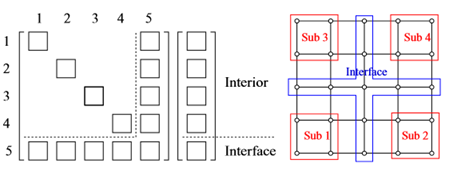
\includegraphics[width=300pt,height=120pt]{SLR.png}
\end{figure}
\T{构造边界方程并求解}
\begin{gather}
		A \begin{bmatrix}
			x \\ y
		\end{bmatrix} = \begin{bmatrix}
			f \\ g 
		\end{bmatrix} \quad A = \begin{bmatrix}
			B & E \\ F & C
		\end{bmatrix} \\ 
		\begin{cases}
			x = B^{-1}(f - E y) \\
			(C - F B ^{-1} E) y = g - F B^{-1} f
		\end{cases}
\end{gather}
\T{构造舒尔补$S=C−FB^{−1}E$需要求解\red{$s$}次$B$
}
\subsection{\T{区域分解类型的预条件子(DD-type Preconditioner)}}
\begin{equation}
	S^{-1} \approx C^{-1}
\end{equation}
\T{预条件子求解仅需求解 \red{2} 次𝐵}

\begin{equation}
	S^{-1} \approx C^{-1} + LRC
\end{equation}
\T{引入矩阵$H$并做近似谱分解}
\[
	H = L^{-1}E^TB^{-1}EL^{-T} \approx UDU^T
\]
舒尔补$S$满足
\begin{itemize}
	\item 
	\begin{equation}
		S = L(I - H)L^T
	\end{equation}
		

	\item 
	\begin{gather}
		\begin{split}
			S^{-1} = L^{-T} (I - H)^{-1}L^{-1} \approx L^{-T} U (I - D)^{-1} U^T L^{-1} \\
			= C^{-1} + L^{-T} U[(I - D)^{-1} - I]U^TL^{-1}
		\end{split}
	\end{gather}
		
\end{itemize}

\section{\T{非对称矩阵稀疏化}}
% .7
\begin{equation}
	A = D + L + U
\end{equation}
\T{将上三角部分和下三角部分分别看成两个无向图}
\T{使用无向图稀疏化 feGRASS}
\T{负数边权值处理为一个极小的正数}
\begin{equation}
	\tag{...\cite{Sparse}}
	M = D + \tilde{L} + \tilde{U}
\end{equation}




\section*{\T{实验与讨论}}
% 1
\begin{figure}[H]
	\caption{\T{实验结果: 对称正定矩阵}}
	\centering
	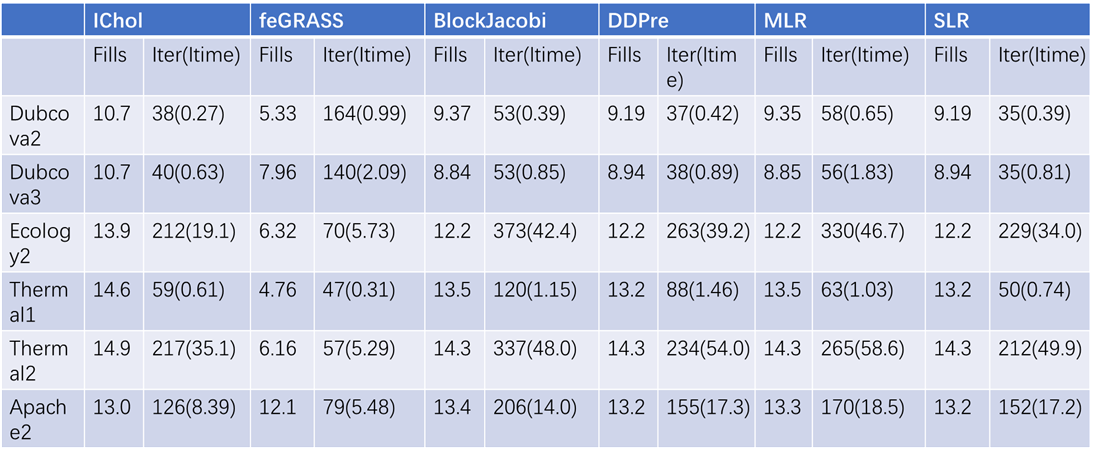
\includegraphics[width=350pt,height=160pt]{SPD_res.png}
\end{figure}
\T{低秩修正技术确实能降低迭代步数,但是能否缩短迭代时间存疑}
\T{在串行意义下,feGRASS效果明显强于其他方法
}

\begin{figure}[H]
	\caption{\T{实验结果: 非对称矩阵}}
	\centering
	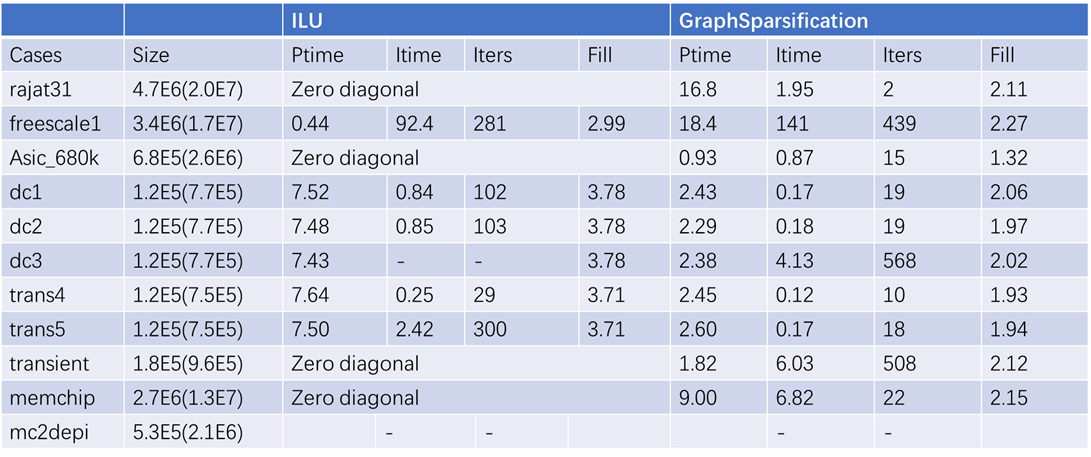
\includegraphics[width=350pt,height=180pt]{normal.png}
\end{figure}

\T{低秩修正技术确实能降低迭代步数,但是能否缩短迭代时间存疑}

\T{在串行意义下,feGRASS效果明显强于其他方法}



\section*{\T{总结}}
% .5
\T{针对对称正定矩阵,比较了六种预条件子}
\T{主要是学习了低秩修正技术}
\T{目前并未实现并行}

\T{针对非对称矩阵,尝试了基于feGRASS的稀疏化方法}
\T{效果一般}


\renewcommand{\refname}{\T{参考文献}}
\bibliographystyle{plain}
\bibliography{参考文献.bib}

\end{document}

